\documentclass[11pt]{jarticle} 

\usepackage[dvipdfmx]{graphicx} % 画像を使うためのパッケージ
\usepackage{amsmath, amsfonts} % 数式を使うためのパッケージ
\usepackage{bm} % 太字の数式を使う
\usepackage{fancyhdr}
\usepackage{wrapfig} %図に対して文章をを回り込ませるfigure

\setlength{\oddsidemargin}{-10mm} % 紙の左のマージン
\setlength{\evensidemargin}{-10mm} % 紙の右のマージン
\setlength{\textwidth}{180mm} % テキストの幅 を指定

\setlength{\topmargin}{-15mm} % 紙の上のマージン
\setlength{\textheight}{255mm} % テキストの高さ

\lhead{東京科学大学 学士特定課題研究 中間報告書} %ヘッダ左
\chead{\empty} %ヘッダ中央
\rhead{提出日:2025年8月1日} %ヘッダ右.コンパイルした日付を表示
\lfoot{\empty} %フッタ左
\cfoot{\thepage} %フッタ中央.ページ番号を表示
\rfoot{\empty} %フッタ右

\pagestyle{fancy}

% ここから本文
\begin{document}

% --------------------------------------------------------

\title{段階的な計算空間の最小化による\\離散制御器合成における計算空間爆発抑制手法}
\author{山口 友輝 (22B30862) \;\; 指導教員:鄭 顕志}
\date{\empty} % 日付は自動的に今日の日付が入る
\maketitle % 上で指定した title と authorを出力
\thispagestyle{fancy}

% --------------------------------------------------------

\section{概要} 
本研究では,離散制御器合成における計算空間の爆発の課題に対処するため,LTSの等価性に基づく最小化を活用した合成手法を提案する.
LTSの等価性とは,同じ事象列を再現できるLTS同士を等価とみなす性質であり,この性質から離散制御器合成過程で構築された多くのLTSは状態数が最小の等価LTSへ変換することが可能である.
本研究では,この最小化を離散制御器合成に導入することで,計算空間の削減を図る.

% --------------------------------------------------------

\section{離散制御器合成を用いた動作仕様設計}

\begin{wrapfigure}{r}[0pt]{0.6\textwidth}
  \centering
  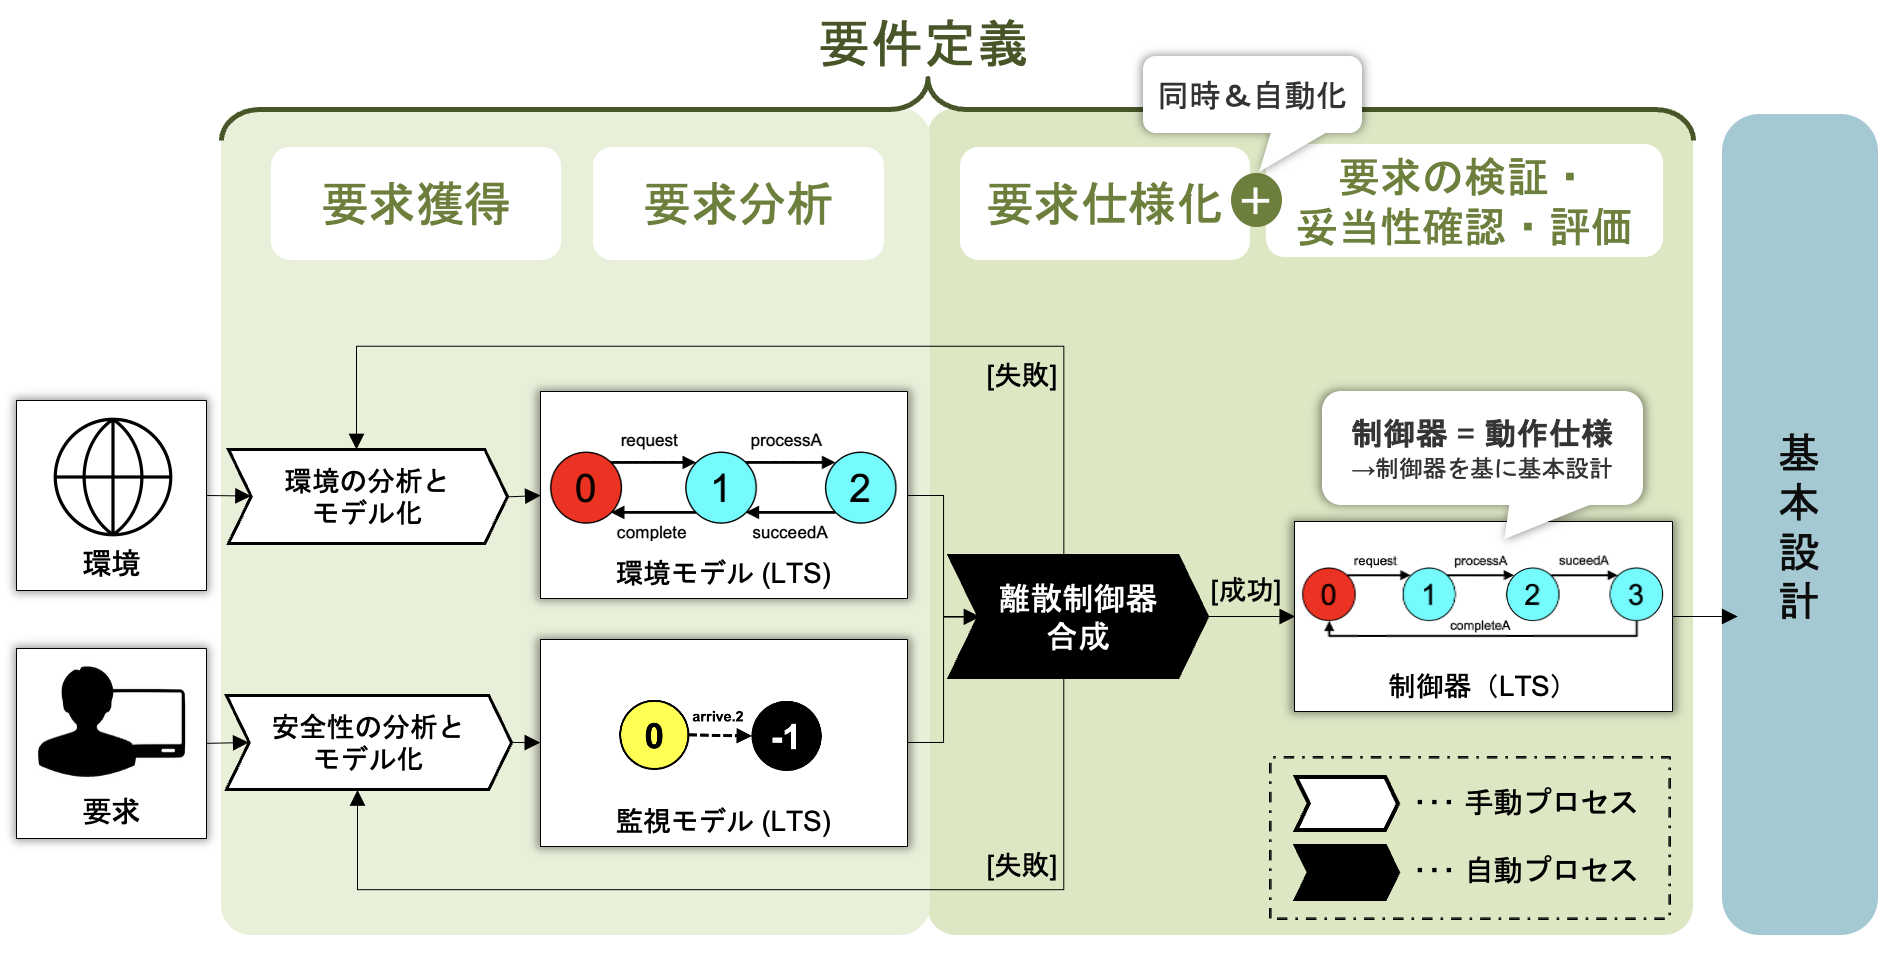
\includegraphics[width=10.8cm]{./figures/DCS.png}
  \caption{離散制御器合成を用いた動作仕様策定}
  \label{fig:1}
\end{wrapfigure}

% 離散事象システムにおける動作仕様設計の説明
事象の発生によりシステムの状態が離散的に遷移する離散事象システムの開発では,開発の早期段階である要件定義において安全性が保証された動作仕様を定めることが重要となる\cite{rebok}.
開発時に想定される動作環境下において安全性が保証された動作仕様を自動合成する技術として,離散制御器合成\cite{concurrency}の研究が進められてきた.

% DCSによる動作仕様設計工程の説明
離散制御器合成を用いた動作仕様設計は図\ref{fig:1}の手順で行われる\cite{concurrency}.はじめに,開発者はシステムの動作環境を仮定し,その特性を環境モデルとしてLabelled Transition Systems(LTS)でモデル化する.次に,環境モデル下で保証すべき安全性を定義し,その安全性の充足状況を監視する監視モデルをLTSで作成する.最後に,環境モデルと監視モデルを入力として離散制御器合成を実施し,環境下で安全性が保証された動作仕様を表すLTSを制御器として自動合成する.

% 関連研究に対する位置付け
安全性が保証された動作仕様を定める技術としては,離散制御器合成以外にもモデル検査やソフトウェアテストが存在する.
対して,離散制御器合成は,モデル検査やソフトウェアテストにおいて繰り返し手動で行われていた動作仕様策定と検証を自動化し,開発者の負担軽減と確実な安全性保証を実現する.

% --------------------------------------------------------

\section{離散制御器合成における課題}
% 離散制御器合成における状態爆発について
しかし,離散制御器合成には計算空間が指数関数的に増加する課題があり,実践的な規模のシステム開発への適用を困難にしている.
離散制御器合成は,制御器を合成する過程で環境モデルと監視モデルから安全性を満たす状態空間を分析するためのゲーム空間を構築する.
ゲーム空間は,事象の同期を考慮した環境モデルと監視モデルの全状態の直積により状態を構築するため,各モデル数の増加に伴って状態数が指数関数的に増加する.
このゲーム空間の指数関数的増加に伴って,要求される計算空間,計算時間,必要主記憶量も指数関数的に増加するため,離散制御器合成において計算空間の状態削減は重要な課題となっている.

% --------------------------------------------------------

\section{LTSの等価性を考慮した離散制御器合成の計算空間削減}
\begin{wrapfigure}{r}[0pt]{0.35\textwidth}
  \centering
  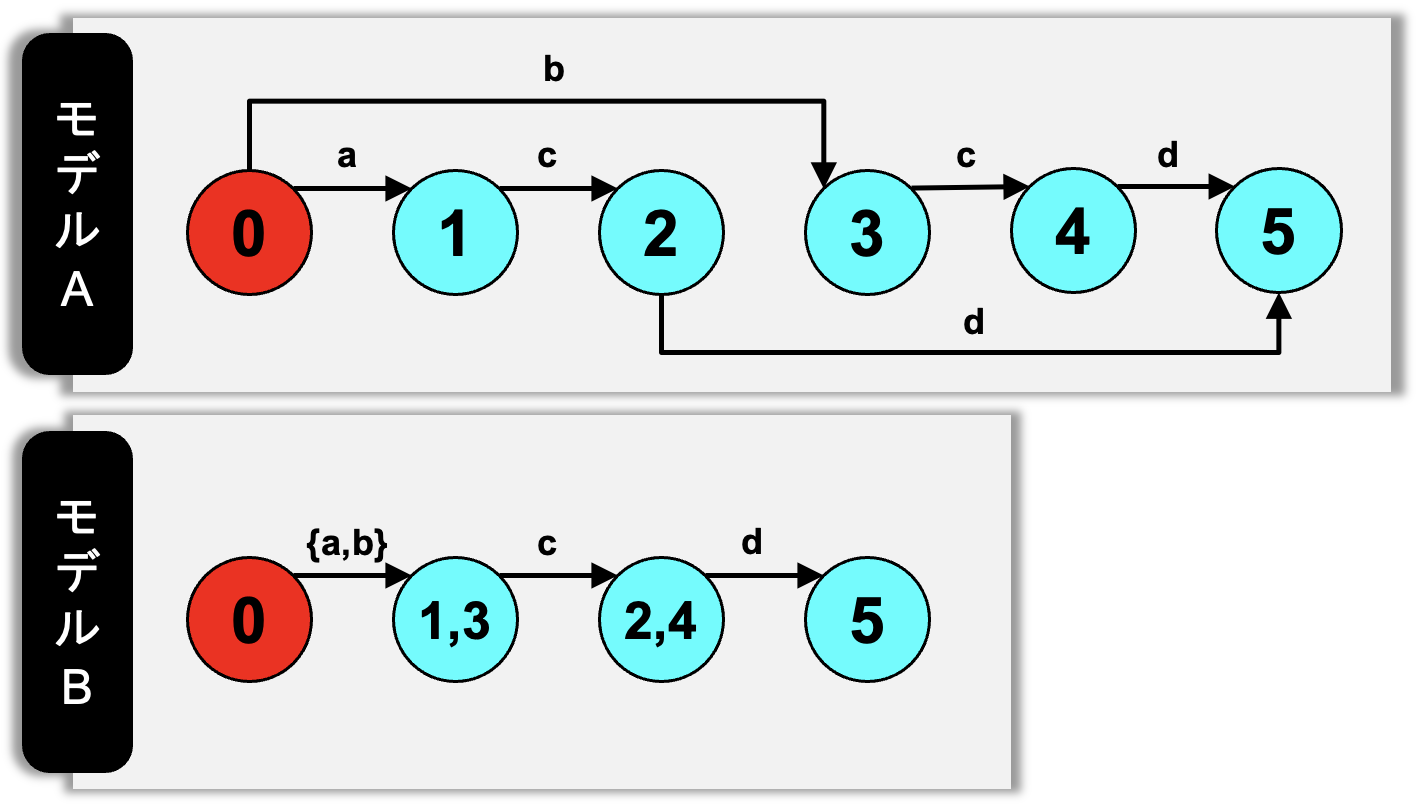
\includegraphics[width=6.3cm]{./figures/minimise.png}
  \caption{等価なLTS}
  \label{fig:2}
\end{wrapfigure}

本研究では,離散制御器合成における計算空間爆発に対処するため,LTSの等価性を考慮した離散制御器合成の計算空間削減に取り組む.

% 状態の等価性について
LTSの等価性とは,あるLTSの初期状態から生成されるすべての事象列を,他のLTSでも再現できるときに,それらが等価とみなせる性質である.
図\ref{fig:2}にはモデルA,Bと名付けられた二つのLTSが示されている.この時,二つのLTSは全く同じ挙動を表し,初期状態0から$a \rightarrow c \rightarrow d$,もしくは$b \rightarrow c \rightarrow d$と遷移することで,状態5に到達する.
この時,モデルAとモデルBは離散制御器合成を行うにあたって等価なLTSとされるが,LTSの状態数がモデルAで6,モデルBで4と異なる.
本研究では,この離散制御器合成におけるLTSの等価性に着目し,離散制御器合成過程で構築される計算空間において,等価なLTSのうち状態数最小となるLTSを扱うことで計算空間が削減できると考えた.

本研究では,あるLTSを状態数最小となる等価なLTSに変換する技術である最小化を,離散制御器合成技術のひとつである段階的離散制御器合成\cite{yamauchi}の計算空間構築過程で活用する.その概要が図\ref{fig:3}である.
段階的離散制御器合成\cite{yamauchi}は,監視モデルごとに必要最小限の構成でゲーム空間の構築と分析を行う部分合成を提案した.そして,部分合成によって安全性を違反すると判明した状態を,他の監視モデルの部分合成において構築回避しつつ,段階的にゲーム空間を構築することで計算空間を削減する.本研究では,部分合成で合成されたLTSに対して最小化を適用し,最小化で削減された状態を以降の部分合成で構築回避する.これにより,最大となる計算空間の状態数を段階的離散制御器合成からさらに削減する.

\begin{figure}[h]
  \centering
  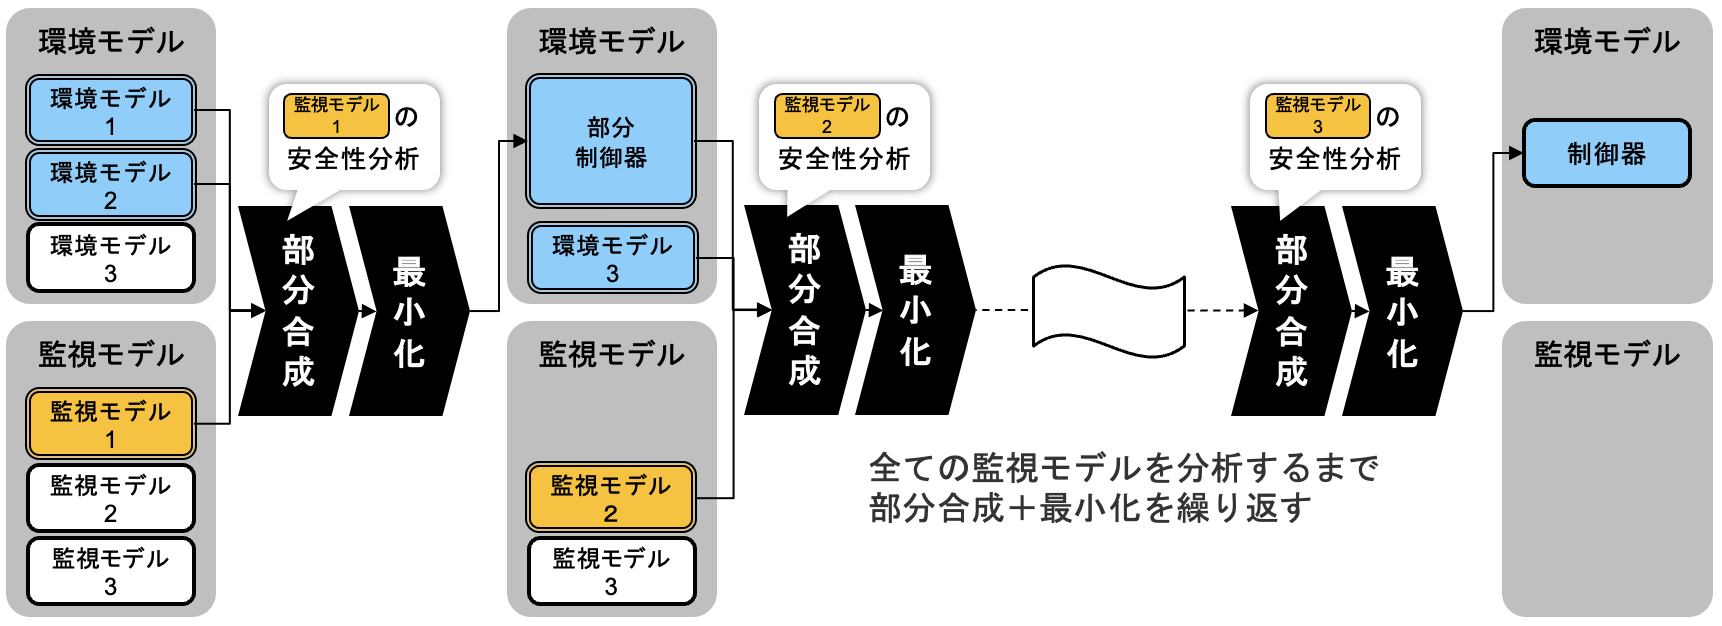
\includegraphics[width=14.5cm]{./figures/proposal.png}
  \caption{計算空間の最小化を活用した段階的離散制御器合成}
  \label{fig:3}
\end{figure}

% --------------------------------------------------------

\section{卒業論文までの研究計画}
現在までに,提案手法の実装は概ね完了している.
今後は,8月中に本手法の有効性を検証するための評価実験を実施する予定である.
評価結果をもとに,9月にはソフトウェア工学分野の研究会であるSIG-KBSEへの論文投稿を目指す.
論文が採択された場合,11月に開催される同研究会において研究成果の発表を行う.
12月から翌年1月にかけては,これまでの研究内容を取りまとめ,卒業論文の執筆を進める計画である.

% --------------------------------------------------------

\begin{thebibliography}{99} % 文献リスト一覧はこんな風に始める
{\footnotesize

\bibitem{rebok}
要求工学知識体系 REBOK: Requirements Engineering Body Of Knowledge, 第1版, 2011, 近代科学社

\bibitem{concurrency}
J.~Magee and J.~Kramer, 
{\it Concurrency: State Models and Java Programs}, 2006.

\bibitem{yamauchi} 
山内拓人, 鄭顕志, 段階的な部分合成による離散制御器合成の分析空間削減, 
IEICE, Vol.~J106-D, No.~4, pp.~218--230, 2023.

}
\end{thebibliography} % 文献リストの最後に必要

% --------------------------------------------------------

\end{document} % 最後の締めくくり。絶体必要